\section{Context}
This thesis sprung from the participation of a team of students to the the Robocup competition, a robotics competition where robots play football.

The ultimate goal of Robocup is to create a team of robots able to beat human champions in football by 2050, as illustrated by the following quote :
\begin{quote}
By the middle of the 21st century, a team of fully autonomous humanoid robot soccer players shall win a soccer game, complying with the official rules of FIFA, against the winner of the most recent World Cup.
\end{quote}

Our team will participle in the kidsize category of the humanoid part of the contest. This means we will have to build a humanoid robot, for the first time at the Montefiore Institute.

\begin{figure}[htp]
\center
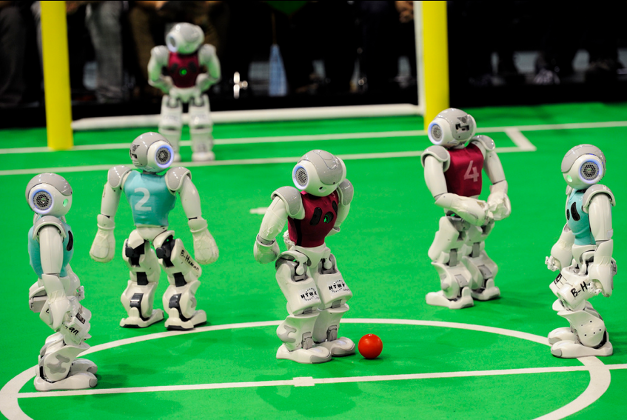
\includegraphics[width=0.5\textwidth]{figures/robocup}
\caption[Two teams of Nao robots playing against each other]{Two teams of Nao robots playing against each other in the 2014 edition of RoboCup \textit{[Photo courtesy of RoboCup]}}
\label{fig:intro_robocup}
\end{figure}

\section{Specifications}
The goal of this thesis is to provide the team with a simulation tool and a model able of :
\begin{itemize}
\item realistically simulating the dynamics of the robot including springs and dampers
\item receiving orders at approximately 300Hz, and we don't really care if the simulation is not in real time.
\item the simulated robot receives exactly the same orders as the real robot would.
\item visualization
\end{itemize}
As the robot is still being designed this thesis should give some insights on how to build it.

\begin{figure}[htp]
\center
\includegraphics[width=0.6\textwidth]{figures/simulation_arch}
\caption[Architecture of the simulation]{Architecture of the simulation}
\label{fig:simul_arch}
\end{figure}
